\documentclass[letterpaper, 10 pt,conference]{ieeeconf}  % Comment this line out if you need a4paper

%\documentclass[a4paper, 10pt, conference]{ieeeconf}      % Use this line for a4 paper

\IEEEoverridecommandlockouts                              % This command is only needed if 
                                                          % you want to use the \thanks command

\overrideIEEEmargins                                      % Needed to meet printer requirements.

% See the \addtolength command later in the file to balance the column lengths
% on the last page of the document

% The following packages can be found on http:\\www.ctan.org
\usepackage{graphicx} % for pdf, bitmapped graphics files
\graphicspath{{../}}
\usepackage{epstopdf} % for postscript graphics files
\usepackage{mathptmx} % assumes new font selection scheme installed
\usepackage{times} % assumes new font selection scheme installed
\usepackage{amsmath} % assumes amsmath package installed
\usepackage{amssymb}  % assumes amsmath package installed
\usepackage[caption=false,font=footnotesize]{subfig}
\usepackage{fixltx2e}
\usepackage{float}

\title{\LARGE \bf
3D-PIV application for autonomous vehicles using monocular vision
}


\author{Eduardo da Silva Afonso$^{1}$ and Fernando Pujaico Rivera$^{2}$ and Arthur de Miranda Neto$^{3}$% <-this % stops a space
\thanks{The authors are with Terrestrial Mobility Lab. at the Federal University of Lavras, Lavras - MG, Brazil.}%
\thanks{$^{1}$  eduardo.afonso@engautomacao.ufla.br, $^{2}$  201518201@posgrad.ufla.br, $^{3}$  arthur.miranda@deg.ufla.br}%
}

\begin{document}


\maketitle
\thispagestyle{empty}
\pagestyle{empty}

\begin{abstract}

In this paper, the Particle Image Velocimetry ($PIV$) technique was adapted to be used in autonomous vehicles.
Applying PIV and the Pearson’s Correlation Coefficient, our proposed algorithm 
is capable of making a three dimensions tracking of the target possible (Region Of Interest) $ROI$ 
and generates a relative departure factor. These data are used to estimate the 
relative velocity of the target ($ROI$) and then analyse the collision risk.

\end{abstract}
\section{INTRODUCTION}

Traffic accident has been an important point to government. The world average of people
died at traffic is around 10 people per 100 thousand, but in countries, like Brazil, it can be worse.
In 2016, the group which compose the UN General Assembly adopted a resolution for
improve global road safety and they consider that 2011-2020 is Decade of Action for Road Safety.
Traffic jam is other problem faced by cities, it is caused by reckless drivers and accidents.
Many centers of research have been studying solutions to improve this condition and decrease the 
numbers of death and accidents.

Monocular vision comes is an emerging field in autonomous vehicles. 
Several application have presented solutions to current problems, 
however systems  of low computational cost remain a challenge. 


The Particle Image Velocimetry ($PIV$)\cite{Bastiaans} technique is used in many fields of 
knowledge, \cite{Story, Xu}, to calculate the velocity of fluids in different parts. 
Here, $PIV$ was adjusted for the case of autonomous vehicles using matching criteria based on 
the Pearson Correlation Coefficient ($PCC$)\cite{Miranda Neto} over the KITTI dataset\cite{Geiger}.

Here, we define some variable used in the paper. The object of interesting is called target.
The region of interesting (ROI) is part of image where the target is and
Window of Search (WOS) is a rectangle where the program will search the ROI. 




\section{THEORETICAL FUNDAMENT}

\subsection{THE PEARSON CORRELATION COEFFICIENT}

$PCC$ is used in statistical analyses, pattern recognition and computer vision. 
It can be used to comparing two images in an object recognition system. 
The following equation describes the $PCC$ method for two gray scale digital images\cite{Eugene},
represented by the matrices $A$ and $B$ with $M$ elements each one,
\begin{equation}
r = \frac{\sum \limits_{i}^{M} (a_i-\mu_a)(b_i-\mu_b)}{\sqrt{\sum \limits_{i}^{M} (a_i-\mu_a)^2} \sqrt{\sum\limits_{i}^{M} (b_i-\mu_b)^2}}.
\end{equation}

where $a_i$ is the intensity of the i-th pixel in the  matrix $A$, 
$b_i$ is the intensity of the i-th pixel in the matrix $B$, 
$\mu_a$ is the mean intensity of $A$,
$\mu_b$ is the mean intensity of $B$ and
$r$ is the correlation coefficient \cite{Miranda Neto}.


\subsection{PARTICLE IMAGE VELOCIMETRY}

$PIV$ is a technique to determine a velocity field from a stream of consecutive 
images of seeded flows\cite{Bastiaans}.
This result is given as a vector field, demonstrating direction, sense and 
intensity of velocity in each particle. 
Moreover, it is possible to calculate rapidly the velocities of any part of image.
For this purpose, the $PIV$ technique divides the image in analysis regions (particles), 
and are searched similarities to these particles in the next image; 
when matches are found, displacement vectors (vector field) are returned,
the analysis regions are refresh and the process is repeated with the consecutive image.



\section{SYSTEM DESCRIPTION}
The purpose of our algorithm is to make a three dimensions tracking system, producing position informations 
about a followed target.
The information will be relevant to define parameters 
as: the relative velocity, the factor of approaching and of departure.

The proposed algorithm is shown in Fig. \ref{fig:system};
it begins with a key frame image where a initial target ($ROI$) is determined; 
the system then receives a stream of image frames and the tracking system 
enters into looping follow this target in the next frames.

\begin{figure}[bhp]
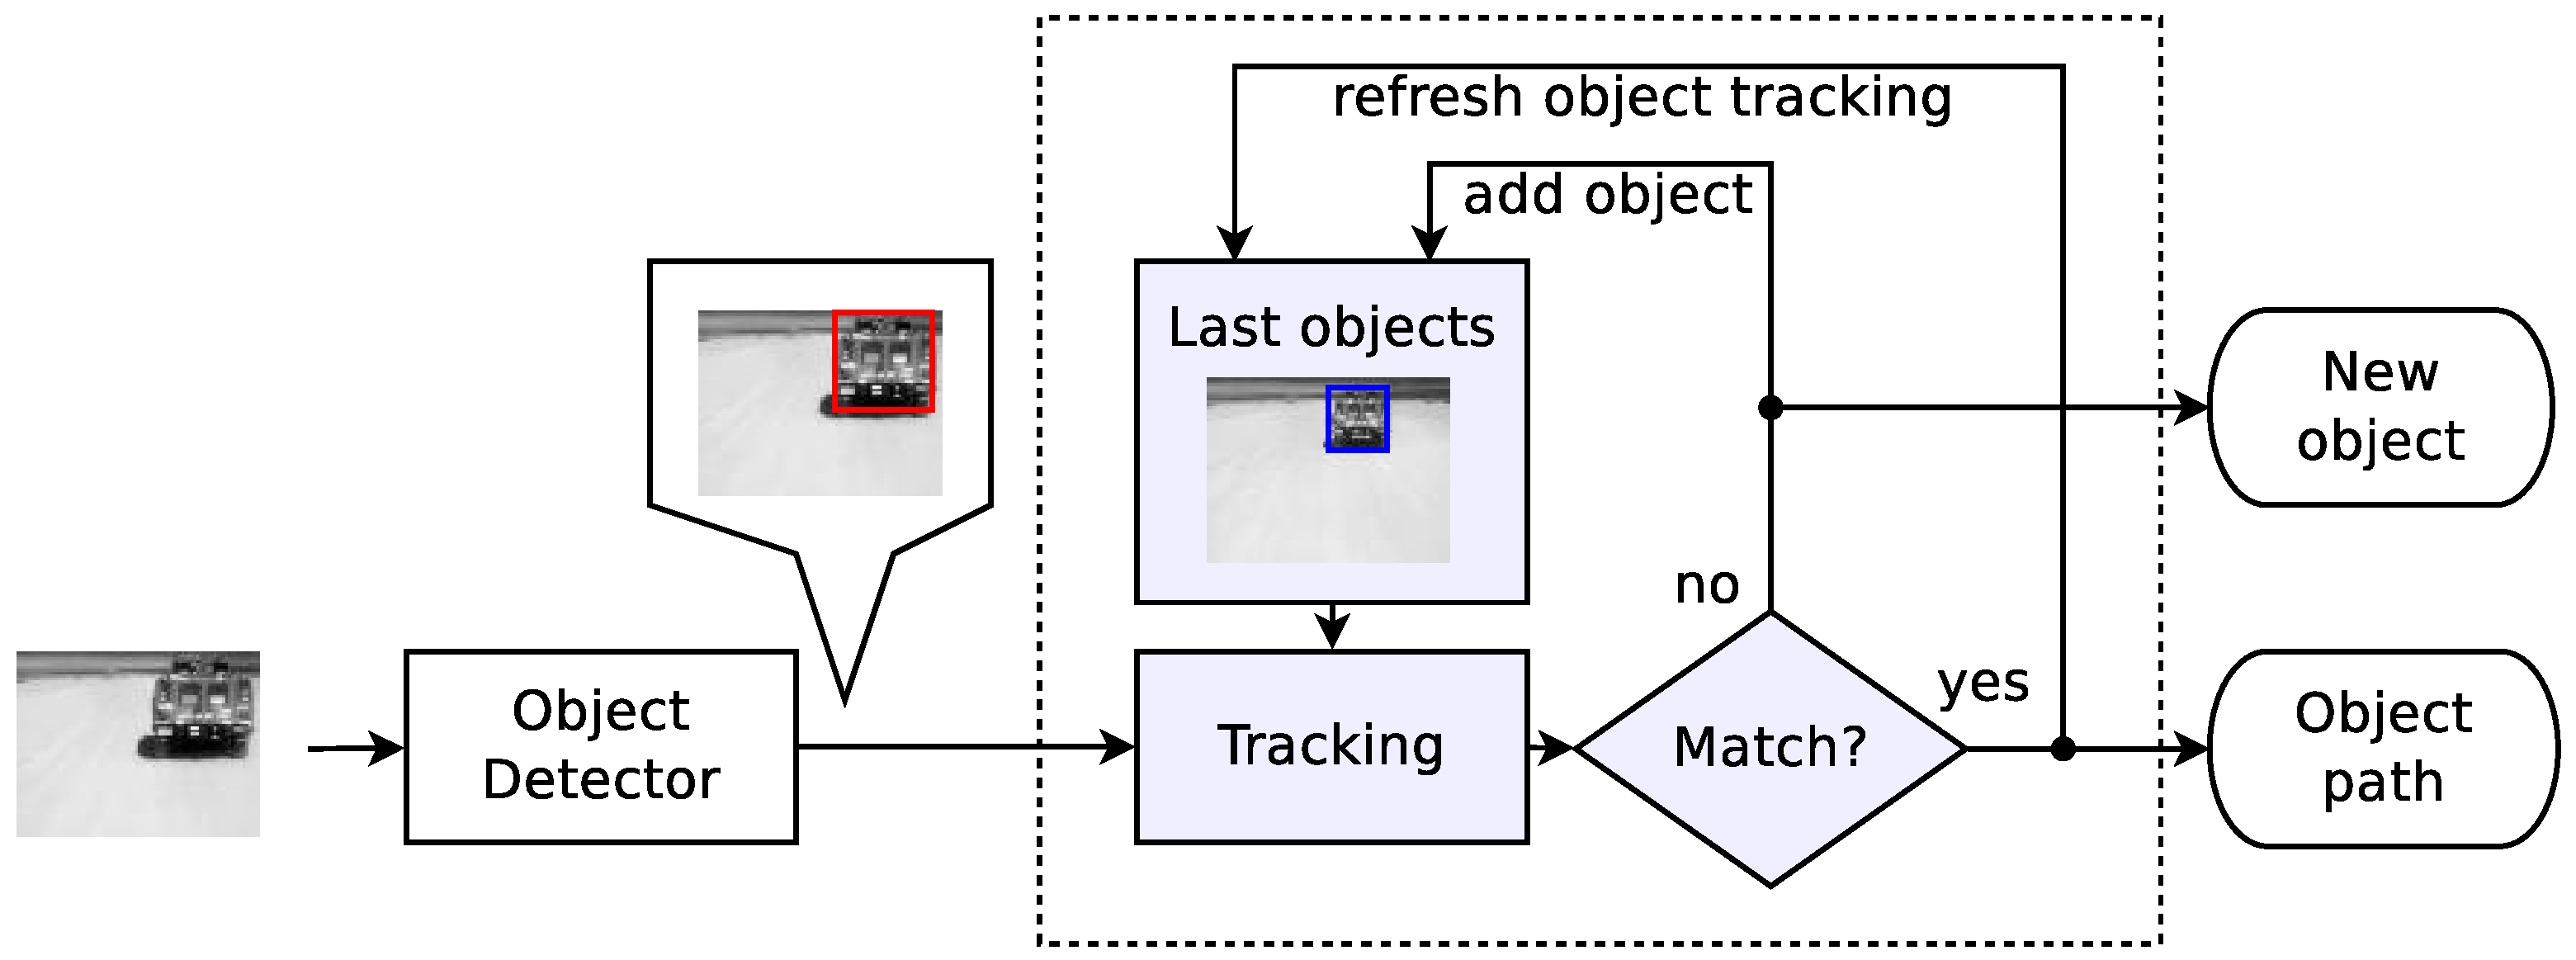
\includegraphics[width=\columnwidth]{images/figure1-diagram1.eps}
\caption{The target is identified from a highest value of correlation (PCC) between a selected ROI and an analysis region in
the $WOS$ of a current frame; the result of this process is a displacement which is  returned as vector field.}
\label{fig:system}
\end{figure}

In a two dimensional analysis, the tracked target given us information about its horizontal 
and vertical position and it is relative to the perpendicular velocity with respect to the observer.
When the target is analyzed in three dimensions, 
the initial $ROI$ has the position $(x=x_0,y=x_0,d=d_0=1)$;
where, $x_0$ and $y_0$ represent a position (horizontal and vertical) in the analyzed image,
and $d_0=1$ represents the initial depth position of target in the $ROI$ (normalized by definition to $1.0$).
Thus, all the results of depth will be relative to this value. In this sense, the relative velocity and 
the factor of approaching or departure can be calculated.

%Diagrama1
 %A gente vai explicar o algoritmo como uma caixa fechada , que coisa entra e que coisa sai
 %e os parametros a sintonizar.
 % como usar ele quando implementado, como se fosse uma caixa preta.


\section{ALGORITHM DESCRIPTION}
 
%DiagramaX

\subsection{MULTI-RESOLUTION MATCH CRITERIA}
Method to track object at image is based on PIV. Figure 2(a) shows the application in 2 dimensions and the next in
3 dimensions.

\begin{figure}[H]
\centering
  \subfloat[]{\label{subfig:(a)} 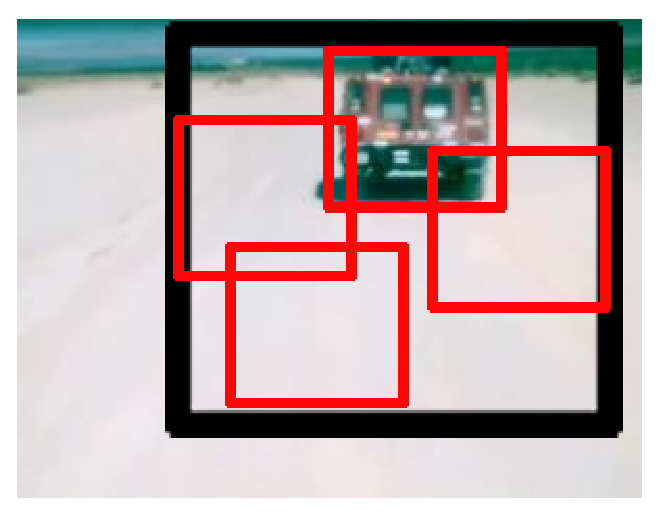
\includegraphics[width=.5\columnwidth]{images/figure2a.eps}}
  \subfloat[]{\label{subfig:(b)} 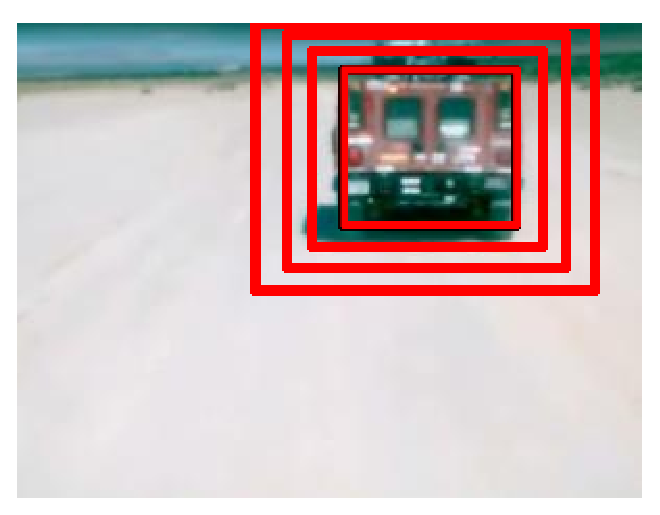
\includegraphics[width=.5\columnwidth]{images/figure2b.eps}}
  \caption{The red box in figure (a) shows the ROI and black box is WOS. In the figure (a), 
  ROI is compared with first portion on the left top of WOS, and these comparisons are made 
  pixel by pixel for whole WOS. The black boxes, in the figure (b), are the WOS used 
  to different layers of search in 3 dimensions}
\end{figure}

To track the object, the ROI defines the size of WOS and, verify the similarity of ROI and parts of WOS using PCC. 
The highest coefficient of Pearson determines new place of object. The figure 2(b) reveals how the dimension of depth was included and, 
the search is made in different layers. In 3 dimensions, the target also is found from the highest PCC among WOS, but the object may be 
bigger or smaller, depending in which layers was.\\
%onde estava, onde esta agora
%que tamanho tinha que tamanho tem.
\subsubsection{MULTI-SCALE 3D INTERPRETATION}
To understand this technique we need to analyse the same target in 
two different positions, as in Fig. \ref{fig:multiscale3d}.

\begin{figure}[H]
\centering
  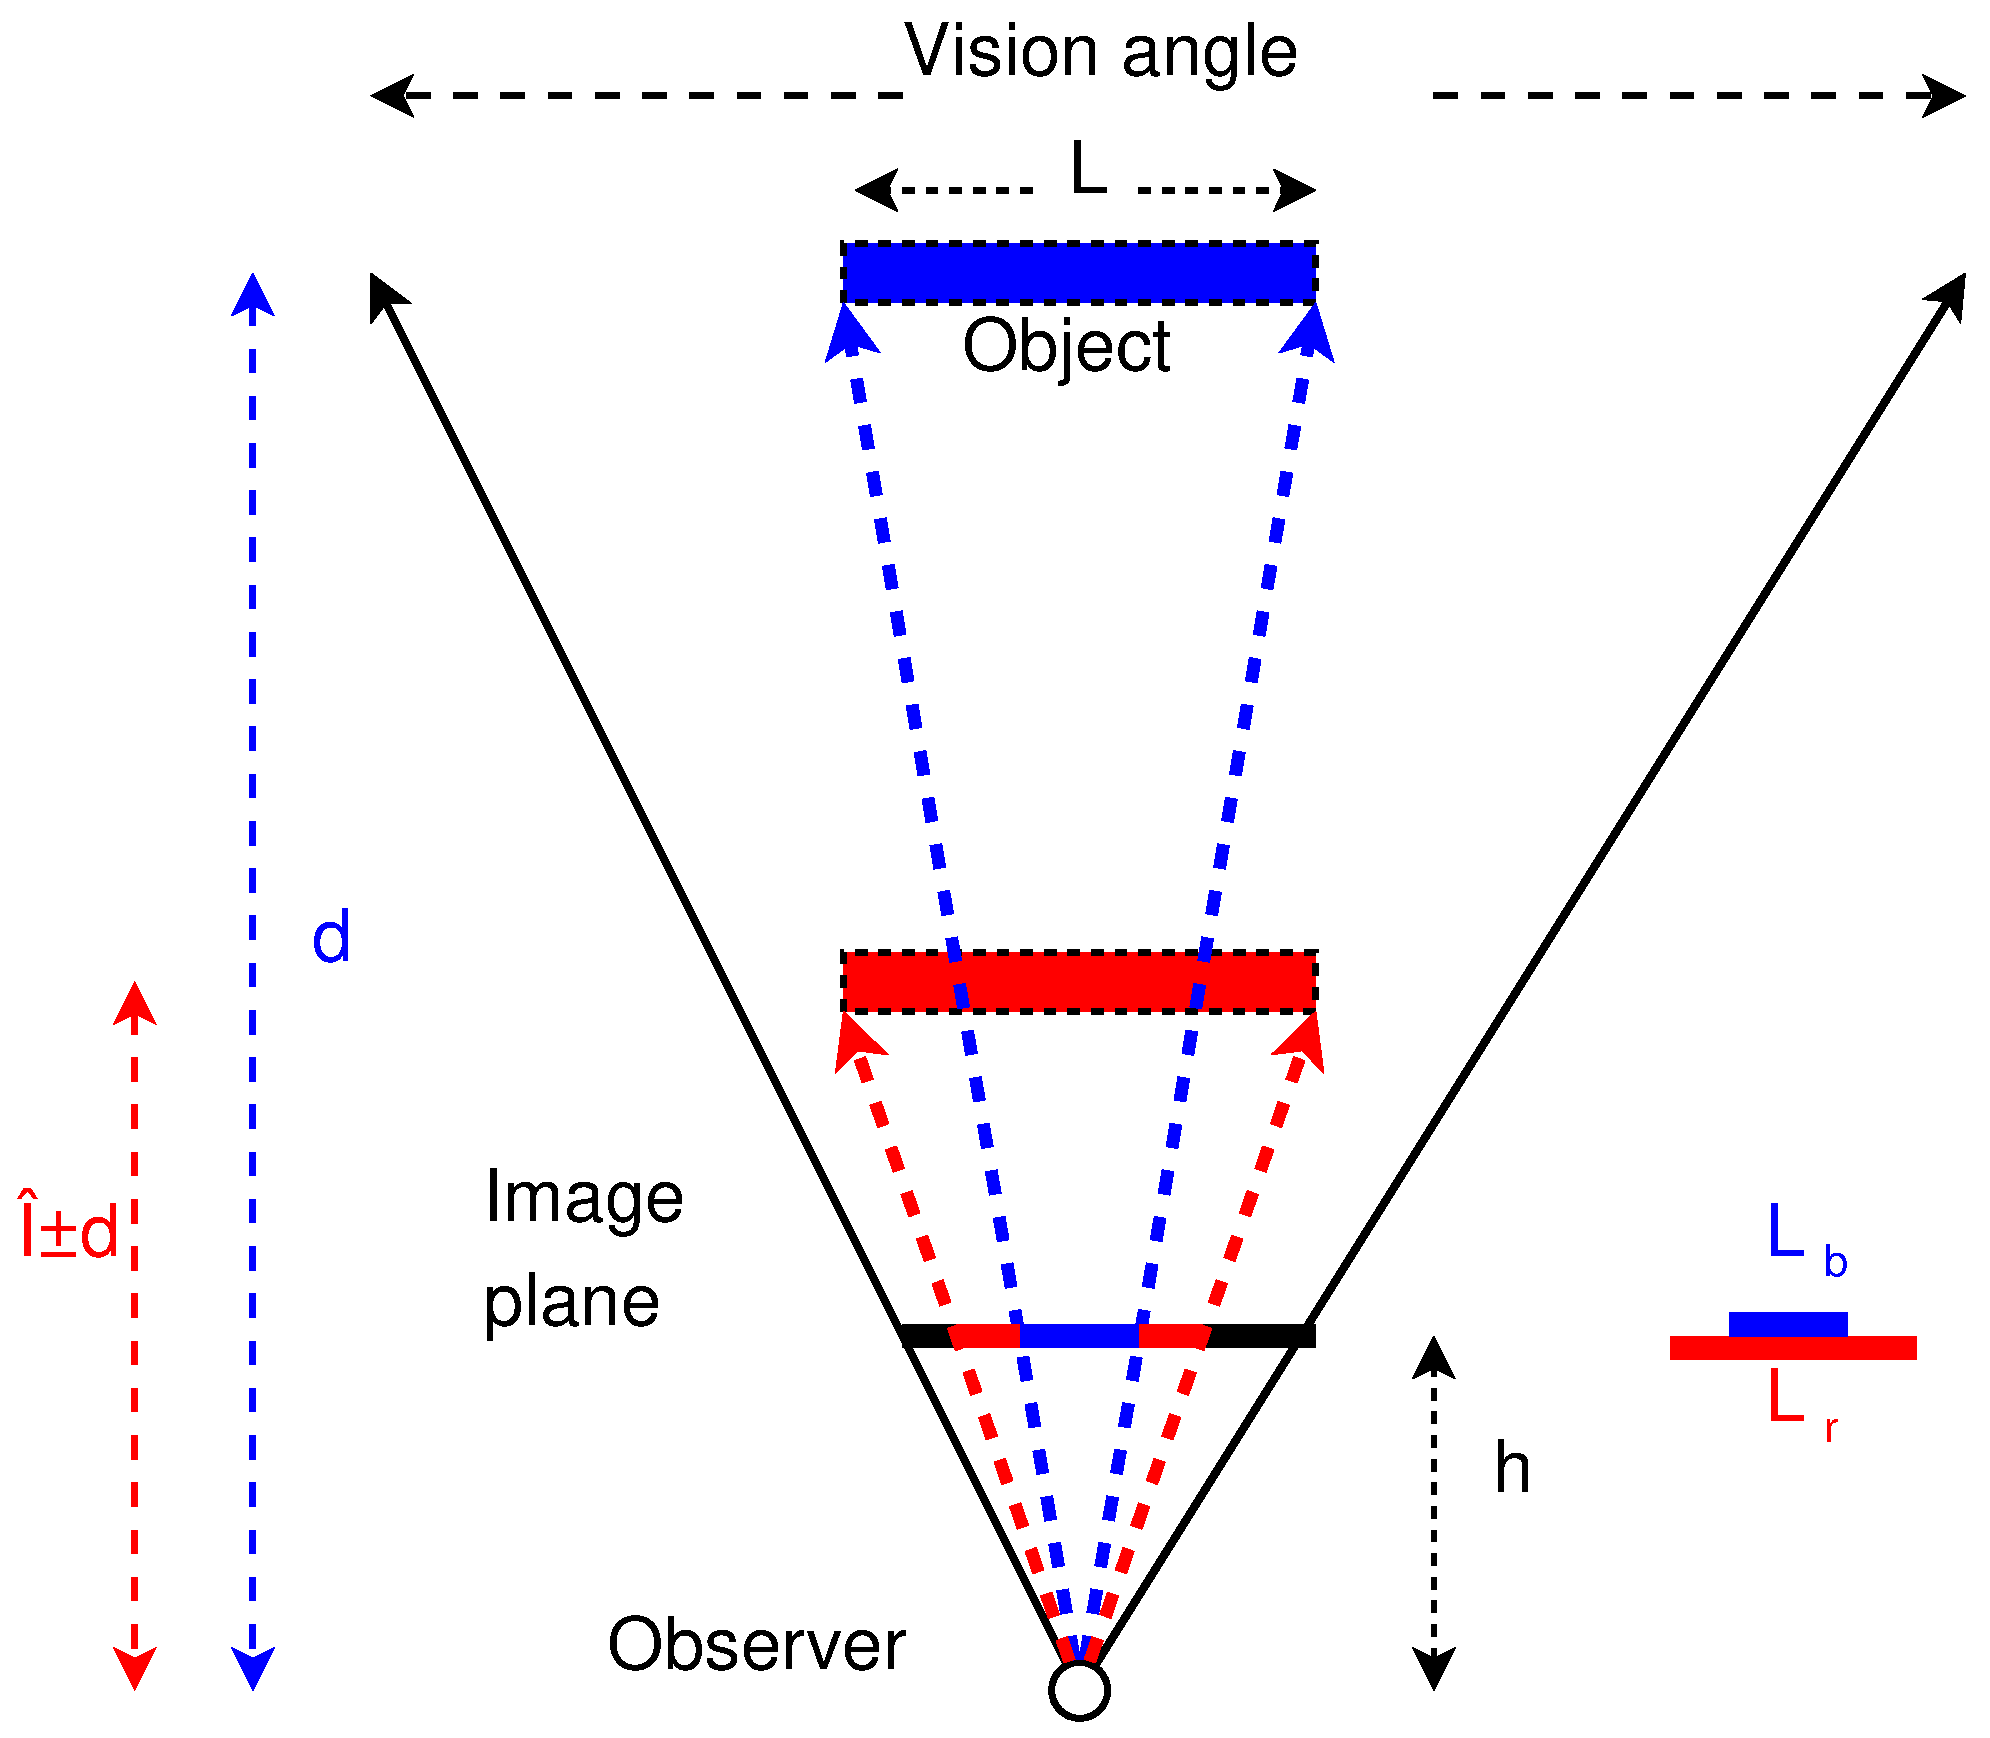
\includegraphics[width=.7\columnwidth]{images/Diagrama3.eps}
  \caption{The multi-scale tracking.}
  \label{fig:multiscale3d}
\end{figure}

Fig.\ref{fig:multiscale3d} shows the same target at two different distances $d$ and $\alpha d$, respectively, in blue and red.
The image plane is located at a distance $h$ of the observer.
The projections of objects, in blue and red, are labelled in the image as
$L_b$ and $L_r$, respectively. Making a simple inspection in the
formed triangles, we can see that $\frac{h}{d}=\frac{L_b}{L}$ and 
$\frac{h}{\alpha d}=\frac{L_r}{L}$, then $L_b/\alpha= L_r$. 
From the point of view of the observer, this implies that when a target 
is located at a distance $d$ at a time $t_0$,  and a distance $\alpha d$ at a time $t_1$, 
the width of the target in the image plane is altered by a factor of 1/$\alpha$, 
and consequently its area is altered by a factor of 1/$\alpha^2$.

The criterion method the searches for objects using different discrete values of $\alpha$. 
The algorithm tracks the nearest objects with $\alpha<1$ and objects farthest with $\alpha>1$.

%usa Multi-resolution match criteria e explica isso dos tamanhos

\subsubsection{DEPARTURE FACTOR - RELATIVE VELOCITY}
The departure factor is a dimensionless number related to the rate of approach 
or departure of a target to the observer. The factor
is determined in \ref{eq:relarea},

\begin{equation}\label{eq:relarea}
f_a \equiv \alpha^2 \equiv \frac{Area_r}{Area_f} 
\end{equation}

where $f_a$ and $\alpha$ are defined as factor area and departure factor, 
respectively; $Area_r$ is the ROI area and $Area_f$ 
is the analyzed region in the current image frame.

Thus, knowing $\alpha$, if we consider that the target in the $ROI$ was to a distance $d_0$,
then the target in the analysis region will be to a distance of $\alpha d_0$ (or $\sqrt{f_a} d_0$).
So that, each $i-th$ frame will have its own $\alpha_i$ value; where, $d_i=\alpha_i d_0$.

The departure factor, $\alpha_i$, has two interpretations: if the rate of departure increases quickly, 
this  means that the target is departing. If the factor decreases, the 
target is approaching.

The relative velocity is using a simple equation of kinematic in physics:
\begin{equation}
 v_i = \frac{\Delta s}{\Delta t}= \frac{s_i-s_{i-1}}{\Delta t}.
\end{equation}

where the vector $v_i$ represents the relative velocity in the i-th image frame, 
$s_i=(x_i,y_i,d_i)$ is the position of match in the i-th image frame
and $\Delta t$ is the sampling time between image frames.
Additionally, we call velocity of departure factor, $v^d_i$, 
the scalar number which represents the depth component
of the vector $v_i$.

The calculated  $v^d_i$ value is relative, for the simple reason that the distance (depth) between the 
camera (observer) and the target in the instance i-th will be referenced to $d_0$, 
given that the distance of the initial $ROI$ is established by definition to 1.
Finally, in all cases, the position $s_i$ is relative to the observer (a moving reference system).


\subsection{RENEW ROI CRITERIA}
%Diagrama2
The $ROI$ is an important element in the algorithm, because of that this  
will be used as pattern to find a match of tracked object at the current image. 
The  question in this case is to know the best moment to refresh the $ROI$
with a new perspective of object. 
Here, we establish the criteria that when the comparison of images return 
a $PCC$ lower than $0.925$ and greater than $0.8$, then the $ROI$ is changed with the current 
analyzed region and a new position of $ROI$ is establish with $(x_i,y_i,d_i)$. 
Thus, it was adopted as $0.8$ the lower limit to a match case\cite{Eugene},
see Fig. \ref{fig:newroicri}. Values less than $0.8$ cause a  lost object alert.
Finally, it is important to note that if the $ROI$ is changed the new $ROI$ is establish
with the real size of the analyzed region and not with the rescaled version used
in the calculus of the $PCC$.


\begin{figure}[H]
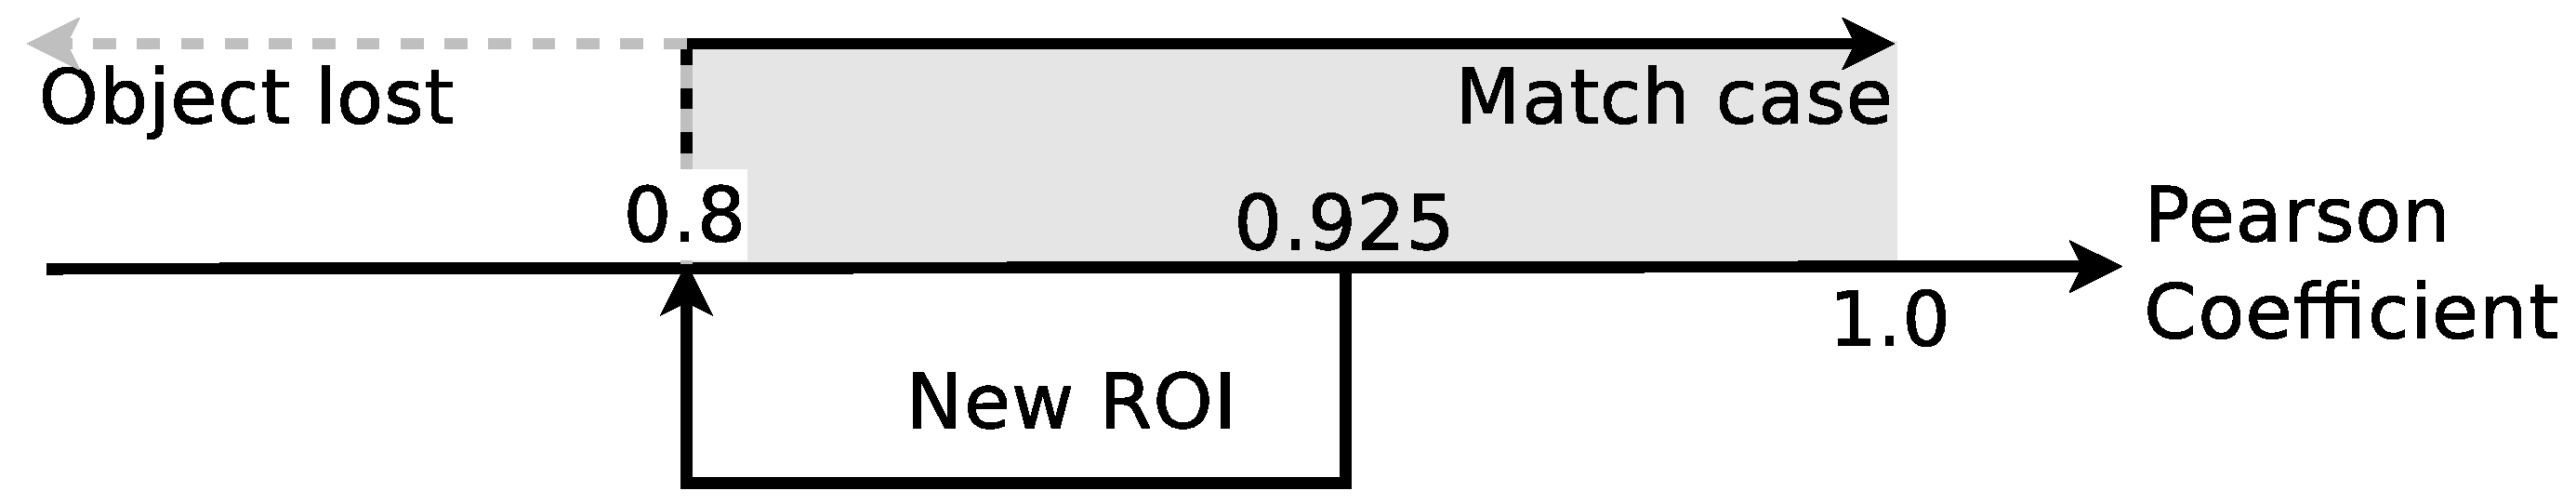
\includegraphics[width=\columnwidth]{images/figure3.eps}
\caption{When the comparison is greater than $0.8$, including numbers bigger than 
$0.925$, means that the target was matched. But if two regions are compared 
and the $PCC$ is less than $0.925$ and greater than $0.8$, 
then the $ROI$ changes to the current analyzed region.}
\label{fig:newroicri}
\end{figure}

The system needs to have high level of reliability, so that the lower limit adopted 
contributes to an operation with minimum of mistakes.


% descrição do sistemA
\section{NUMERICAL RESULTS}
The followed informations introduce the results of two different tests 
using the KITTI dataset\cite{Geiger}.


In the first test in Fig. \ref{fig:imgpapercerta}, 
the algorithm makes the tracking of an object through nine images in sequence with 
a displacement approximately perpendicular to the observer.
\begin{figure}[!hbt]
\centering
  \subfloat[]{\label{fig:imgpapercertaa} \includegraphics[width=.48\columnwidth]{images/images/0000000000.png}}
  \subfloat[]{\label{fig:imgpapercertab} \includegraphics[width=.48\columnwidth]{images/images/img_paper_certa.eps}}
  \caption{The image in (a) represents the target in its initial position 
   and the image (b) shows the vehicle in its final position.}
  \label{fig:imgpapercerta}
\end{figure}
The initial position of target is in the image (a) and the final position in (b), 
where a vector (in blue) illustrates the resulting trace.
We can observe that there is a small bend in the image 
and it generates a slight change of object perspective. 
This cause the update of the $ROI$, which involves seeing a slight change in area.
The difference among the initial and final values of the departure factor may 
be considered small, as shown in Fig. \ref{fig:res_graph1}.
\begin{figure}[!hbt]
\centering
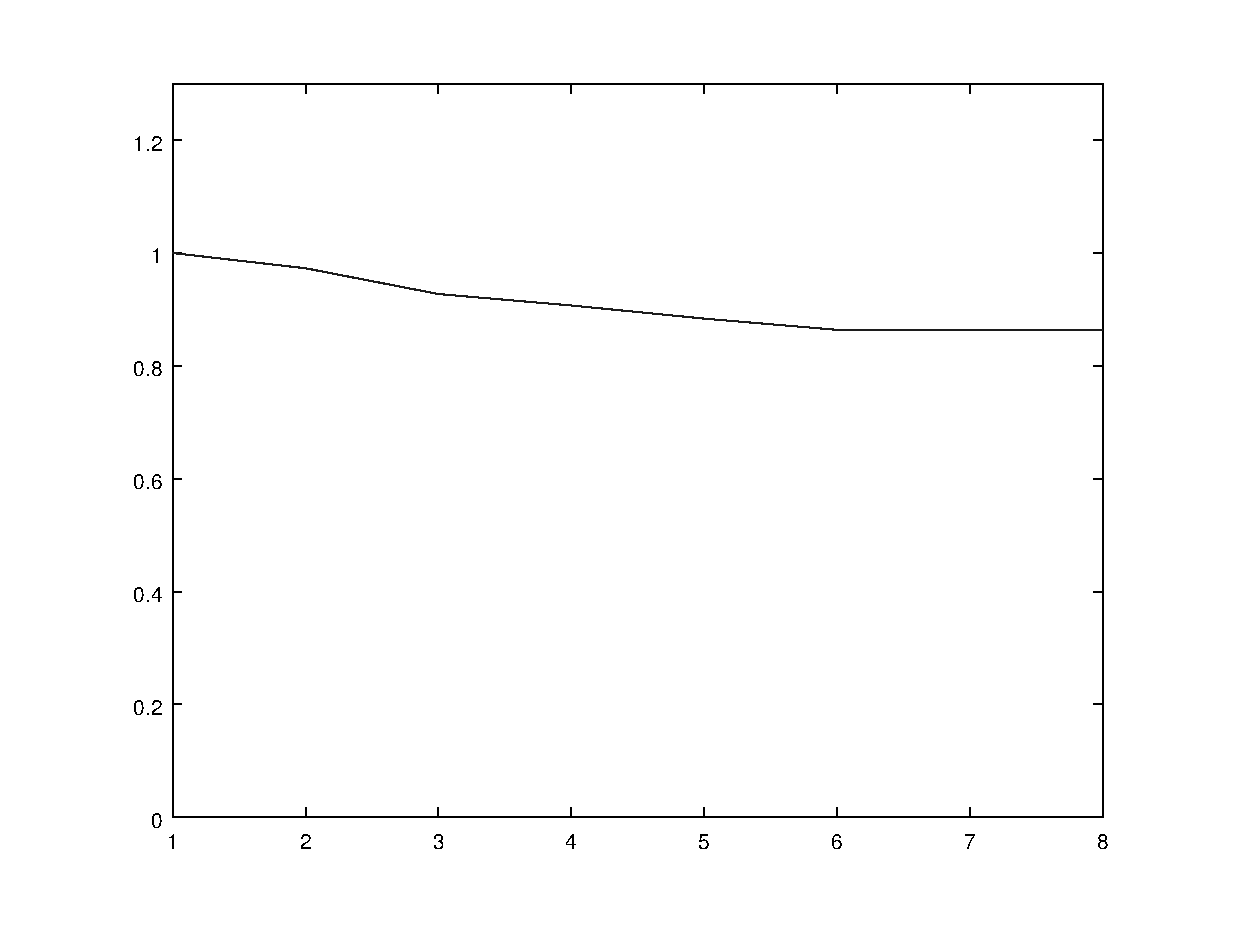
\includegraphics[width=0.8\columnwidth]{images/graph1.eps}
\caption{Departure factor for each frame in the test 1.}
\label{fig:res_graph1}
\end{figure}
Fig. \ref{fig:res_graph1v} shows the velocity of departure factor
to a value $d_0=1$ and a $\Delta t=1$. It demonstrates that the variation
of the departure factor is very small when compared with 1. 
It has a mean departure factor (velocity) of $-0.017020$. This implies in a mean approach of $1.7\%$ of $d_0$
in each one of the nine frames.
\begin{figure}[!hbt]
\centering
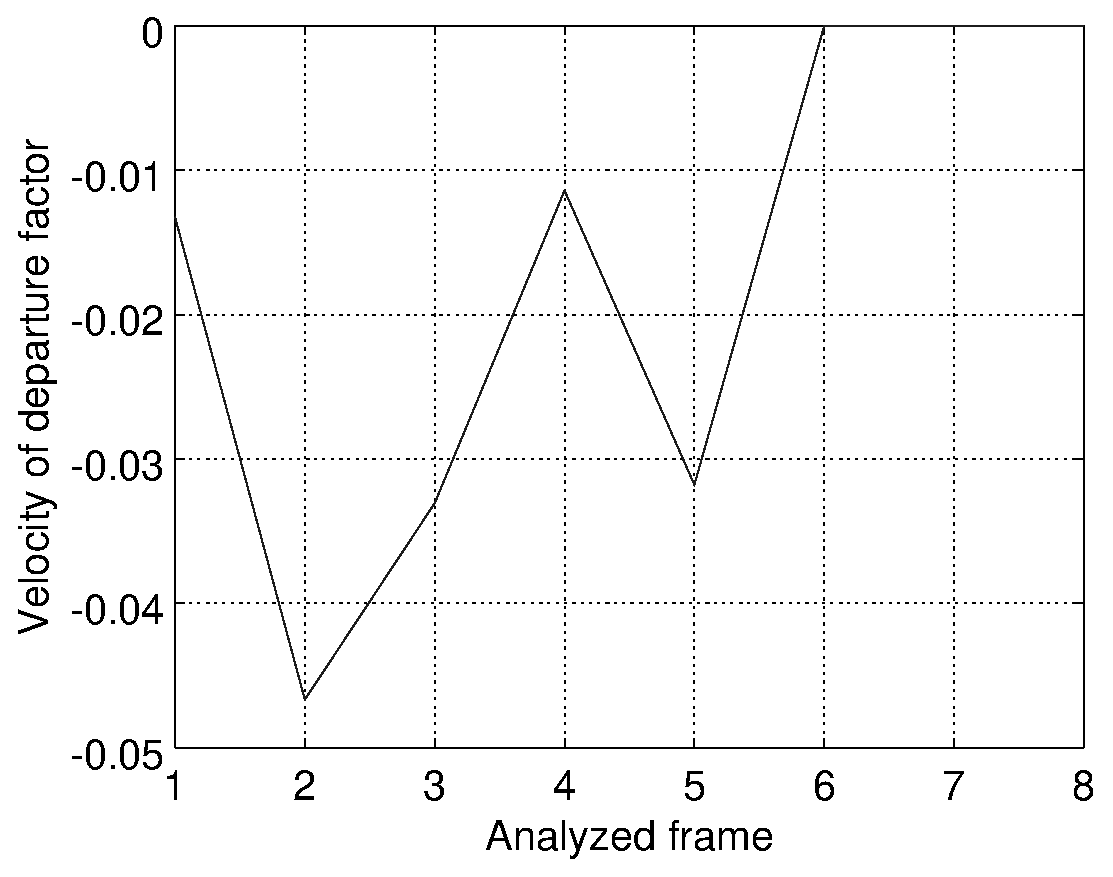
\includegraphics[width=0.8\columnwidth]{images/graph1v.eps}
\caption{Velocity of departure factor for each frame in the test 1.}
\label{fig:res_graph1v}
\end{figure}

%testes com diferentes parametros
% tabelas e graficos

\section{CONCLUSIONS}
From the presented examples,
it can be observed that one application that uses the tracking
and the departure factor is related with the risk of collision.
It is possible to estimate how of fast an object is departing.
Thus, if the  departure factor tends to zero or 
if the velocity of departure factor changes to lower negatives values every time, 
probably, there is a high risk of collision. The $PIV$ technique has presented satisfactory results. 
It can be concluded that estimating collision using velocity of departure factor, 
tracking of objects in 2 or 3 dimensions, and departure distance
relative to the first position of $ROI$. 
The simulations in both cases has given promissory results.

\addtolength{\textheight}{-12cm}

\section*{ACKNOWLEDGMENT}

We want to thank to FAPEMIG, LMT and UFLA for support given to this research.
Project number associated to this research by FAPEMIG: PIDEG37-2015.

%FAPEMIG\\
%numero de bolsa\\
%numero de projeto\\
%numero de aluno


\begin{thebibliography}{99}
	\bibitem{Bastiaans} R. J. M. Bastiaans, Cross-correlation PIV; theory, implementation and accuracy. 
        Eindhoven: Technische Universiteit Eindhoven, 2000. - EUT Report 99-W-OOl. - ISBN: 90-386-2851-X.

	\bibitem{Story} A. Story et al, PIV measurements of the velocity field of a Newtonian Fluid in a stirred tank equipped 
	with the PMT type impeller.Technical Transactions - Chemistry. 2-Ch/2014.        

	\bibitem{Xu} L. Xu, Computational fluid dynamics analysis and PIV validation of a bionic vortex flow 
	pulsatile LVAD.Technology and Health Care 23 (2015) S443?S451. DOI 10.3233/THC-150981. IOS Press, 2015.
	
        \bibitem{Miranda Neto} A. Miranda Neto et al, Image Processing Using Pearson's Correlation Coefficient: 
        Applications on Autonomous Robotics. 
        Autonomous Robot Systems (Robotica), 2013 13th International Conference on, 2013.
        
        \bibitem{Geiger} A. Geiger et al,
        Vision meets Robotics: The KITTI Dataset. International Journal of Robotics Research (IJRR), 2013, 
        doi:10.1177/0278364913491297 .
        
        \bibitem{Eugene} Y. K. Eugene and R.G. Johnston, The Ineffectiveness of the Correlation Coefficient for Image Comparisons.
        Technical Report LA-UR-96-2474, Los Alamos, 1996.
        
        %\bibitem{Auoude} G.S. Auoude et al. Sampling-Based Threat Assessment Algorithms for Intersection Collisions Involving 
        %Errant Drivers. IFAC Symposium on Intelligent Autonomous Vehicles, 2010.
        
        %\bibitem{Jonas} T. Jonas, Real-Time Probabilistic Collision Avoidance for Autonomous Vehicles, Using Order Reductive 
        %Conflict Metrics. Submitted to the Department of Aeronautics and Astronautics
	%in partial fulfillment of the requirements for the degree of Doctor of Philosophy. Massachusetts Institute of Technology. June, 2003.
	
	%\bibitem{Woerner} K. Woerner, COLREGS-Compliant Autonomous Collision Avoidance Using Multi-Objective Optimization
	%with Interval Programming. Submitted to the Department of Mechanical Engineering in partial fulfillment of the requirements for the 
	%degrees of Naval Engineer and Master of Science in Mechanical Engineering. Massachusetts Institute of Technology. June, 2014.

\end{thebibliography}

\end{document}
